\documentclass{lab}

\renewcommand{\AA}{\ensuremath{\mathring{A}}}

\begin{document}

\labtitle{4.5.3}{Сканирующий интерферометр}{10~мая~2019~г.}{16~мая~2019~г.}

\section*{Постановка эксперимента}

\begin{quote}
	\textbf{{\normalsize Цель работы: }}
	знакомство с устройством и работой газового лазера
	непрерывного действия, со спектральными характеристиками лазерного излучения, а также с устройством и принципом действия сканирующего интерферометра Фабри–Перо.
\end{quote}

\begin{quote}
	\textbf{{\normalsize Оборудование: }}
	Не-Nе лазер с блоком питания; сканирующий интерферометр Фабри–Перо; поляроид; пластинка $ \lambda $/4; линза;
	фотодиод; электронный осциллограф.
\end{quote}

\subsection*{Схема установки}

\begin{figure}[H]
	\centering
	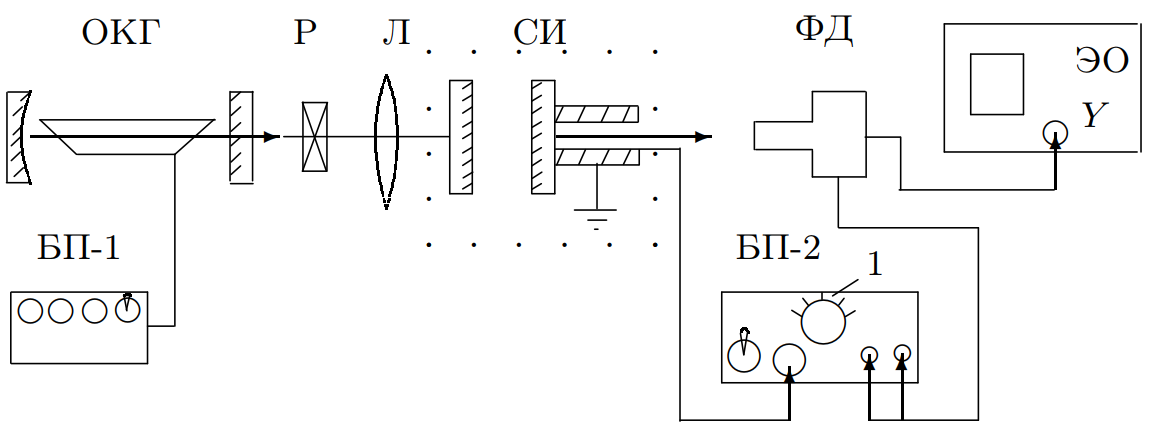
\includegraphics[width = \textwidth]{setup}
	\caption{Схема установки для наблюдения дифракции на акустической решетке}
	\label{scheme}
\end{figure}

Схема экспериментальной
установки приведена на рис. 6. Излучение He-Ne лазера (ОКГ) про
ходит через
поляризационную развязку
Р
и линзу
Л
и поступает на вход сканирующего интерферометра (СИ).

\subsection*{Теоретическая часть}

\begin{equation}
\Delta \nu = \dfrac{c}{2L} ~~~~~~~ \Delta \lambda = \dfrac{\lambda^2}{2L} ~~-~~ интерферометр~внутри~лазера.
\end{equation}

\begin{equation}
\Delta \nu_{СИ} = \dfrac{c}{2l} ~~~~~~~ \Delta \lambda_{СИ} = \dfrac{\lambda^2}{2l} ~~-~~ интерферометр~Фабри-Перо.
\end{equation}

\begin{equation}
R = \dfrac{\lambda}{\delta \lambda} = \dfrac{2\pi l}{\lambda(1-r)}
\end{equation}

\begin{equation}
R = \dfrac{2\pi l \sqrt{r}}{\lambda(1-r)} = Q\sqrt{r}
\end{equation}

\newpage

\subsection*{Выполнение работы}

\begin{equation}
\lambda = 6328 \AA, l = 9~см, L = 55~мм
\end{equation}

\begin{enumerate}
\item
Рассчитаем межмодовое расстояние резонатора ОКГ в единицах $ \lambda  $ и $ \nu  $ по формуле:
\begin{equation}
\Delta \nu = \dfrac{c}{2L} = 273~МГц, ~~~~~~~ \Delta \lambda = \dfrac{\lambda^2}{2L} = 364 \cdot 10^{-5} \AA
\end{equation}

\item 
Подсчитаем число промежутков и оценим видимую ширину спектральной линии Неона:\\
Имеем порядка 7 межмодовых промежутка, тогда:
\begin{equation}
\Delta \lambda(Ne) \approx 7 \cdot \Delta \lambda \approx 2.4 \cdot 10^{-2 } \AA, ~~~~~~~ \Delta \lambda \approx 1900 ~МГц
\end{equation}

\item
Полагая, что ширина спектральной линии обусловлена только эффектом Доплера и что видимая ширина линии Неона порядка полуширины доплеровского контура $ (\Delta \lambda (Ne) \approx \Delta \lambda_D) $, оценим скорость атомов Ne и газокинетическую температуру в разряде.
\begin{equation}
v_x \approx c \dfrac{\Delta \lambda_D}{2 \lambda } = 570~м/с, ~~~~~~~ T \approx \dfrac{m v_x^2 }{k} = 760~К
\end{equation}

\item
Рассчитаем доплеровскую область $ \Delta \lambda_{СИ} $ сканирующего интерферометра:
\begin{equation}
\Delta \lambda_{СИ} = \dfrac{\lambda^2 }{2l } \approx 2.2 \cdot 10^{-2} \AA, ~~~~~~~~~ \Delta \lambda_{СИ} = 1670~МГц
\end{equation}

Полученные результаты довольно точно сходятся с ранее полученными данными.

\item 
Оценим разрешение $ \delta \lambda  $ и разрешающую способность интерферометра:
\begin{equation}
\delta \lambda \approx \dfrac{\Delta \lambda}{5} = 	73\cdot 10^{-5} \AA, ~~~~~~~ R \approx \dfrac{\lambda}{\delta \lambda } = 8.7 \cdot 10^6 
\end{equation}

\item 
Оценим коэффициент отражения зеркал интерферометра:
\begin{equation}
(1-r) = \dfrac{2\pi l}{\lambda R} = \dfrac{\delta \lambda \cdot 2 \pi l}{\lambda^2} \then r = 1 - \dfrac{\delta \lambda \cdot 2 \pi l}{\lambda^2} = 0.897 \approx 0.9
\end{equation}

\end{enumerate}

\subsection*{Итоги}
Изучены интерферометр Фабри-Перо и сканирующий интерферометр. Также оценены различные параметры лазера, резонатора и параметров интерферометра Фабри-Перо.

\begin{equation}
R \approx 0.87\cdot 10^6 ~~~~~ r \approx 0.9 ~~~~~ T \approx 760~K ~~~~~ \Delta \lambda_{СИ} \approx 2.2\cdot 10^{-5} \AA ~~~~~ \Delta \nu _{СИ} \approx 1670~МГц
\end{equation}

\end{document}